\documentclass{standalone}
\usepackage{tikz}
\usetikzlibrary{patterns, positioning}


\begin{document}
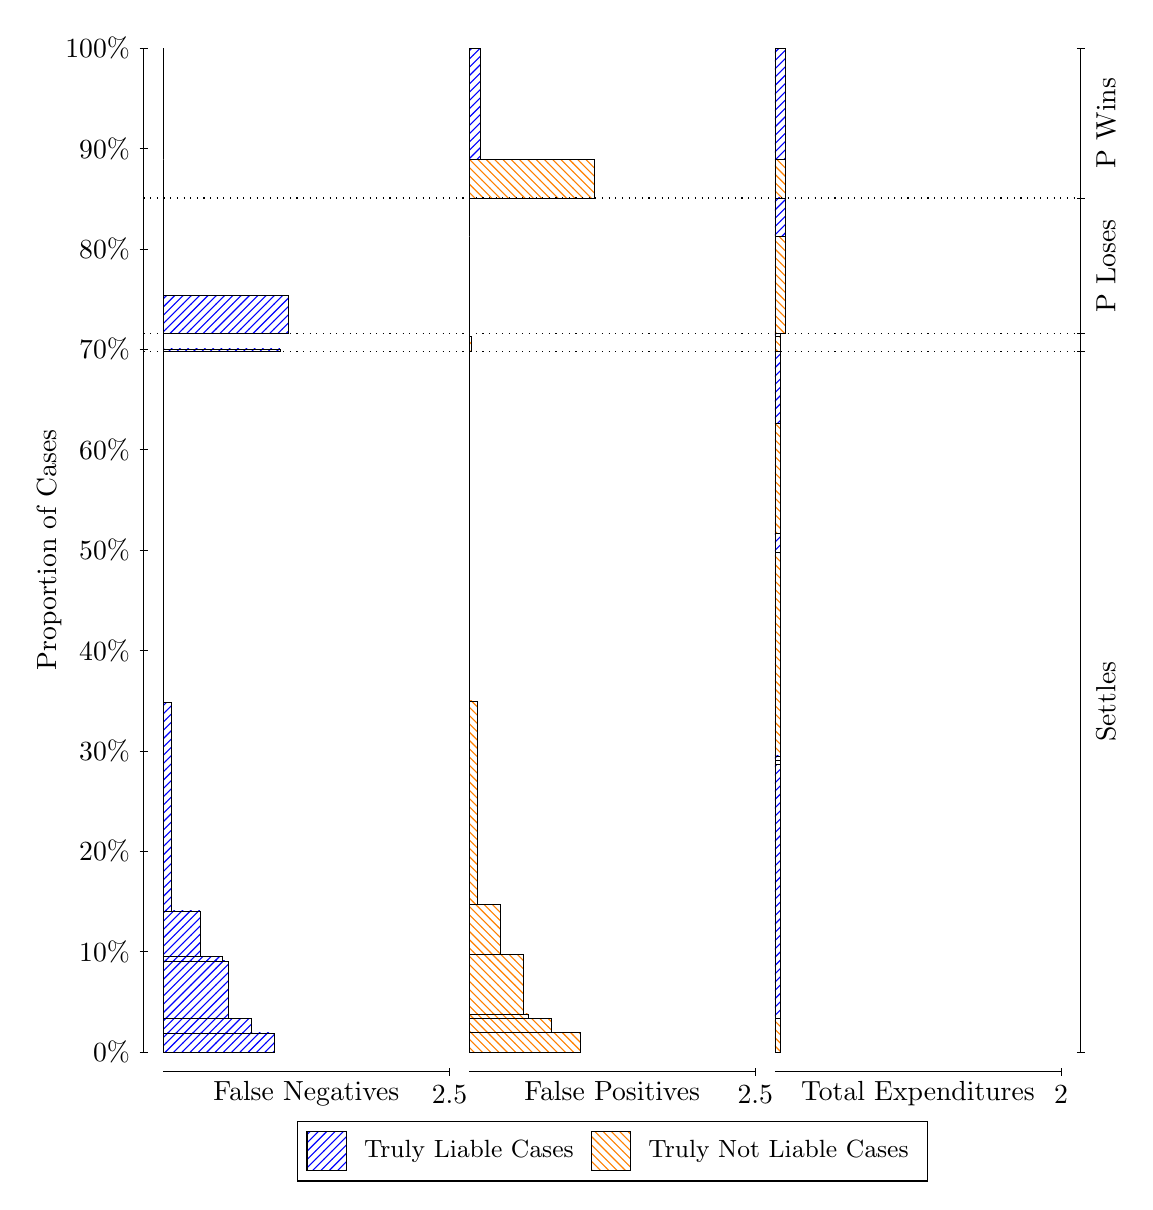
\begin{tikzpicture}
\draw[black, very thin] (1.5,1.75) -- (1.5,14.5);
\node[rotate=90, text=black, anchor=center] at (0.3, 8.125) {Proportion of Cases};
\draw[black, very thin] (1.45,1.75) -- (1.55,1.75);
\node[text=black, anchor=east] at (1.45, 1.75) {0\%};
\draw[black, very thin] (1.45,3.025) -- (1.55,3.025);
\node[text=black, anchor=east] at (1.45, 3.025) {10\%};
\draw[black, very thin] (1.45,4.3) -- (1.55,4.3);
\node[text=black, anchor=east] at (1.45, 4.3) {20\%};
\draw[black, very thin] (1.45,5.575) -- (1.55,5.575);
\node[text=black, anchor=east] at (1.45, 5.575) {30\%};
\draw[black, very thin] (1.45,6.85) -- (1.55,6.85);
\node[text=black, anchor=east] at (1.45, 6.85) {40\%};
\draw[black, very thin] (1.45,8.125) -- (1.55,8.125);
\node[text=black, anchor=east] at (1.45, 8.125) {50\%};
\draw[black, very thin] (1.45,9.4) -- (1.55,9.4);
\node[text=black, anchor=east] at (1.45, 9.4) {60\%};
\draw[black, very thin] (1.45,10.675) -- (1.55,10.675);
\node[text=black, anchor=east] at (1.45, 10.675) {70\%};
\draw[black, very thin] (1.45,11.95) -- (1.55,11.95);
\node[text=black, anchor=east] at (1.45, 11.95) {80\%};
\draw[black, very thin] (1.45,13.225) -- (1.55,13.225);
\node[text=black, anchor=east] at (1.45, 13.225) {90\%};
\draw[black, very thin] (1.45,14.5) -- (1.55,14.5);
\node[text=black, anchor=east] at (1.45, 14.5) {100\%};

\draw[black, very thin] (13.4,1.75) -- (13.4,14.5);
\draw[black, very thin] (13.35,1.75) -- (13.45,1.75);
\node[anchor=west] at (13.35, 1.75) {};
\draw[black, very thin] (13.35,10.645) -- (13.45,10.645);
\node[anchor=west] at (13.35, 10.645) {};
\draw[black, very thin] (13.35,10.872) -- (13.45,10.872);
\node[anchor=west] at (13.35, 10.872) {};
\draw[black, very thin] (13.35,12.596) -- (13.45,12.596);
\node[anchor=west] at (13.35, 12.596) {};
\draw[black, very thin] (13.35,14.5) -- (13.45,14.5);
\node[anchor=west] at (13.35, 14.5) {};

\draw[black, very thin, pattern color=blue, pattern=north east lines] (1.75,1.75) rectangle (3.1579,1.9925);
\draw[black, very thin, pattern color=blue, pattern=north east lines] (1.75,1.9925) rectangle (2.8673,2.1779);
\draw[black, very thin, pattern color=blue, pattern=north east lines] (1.75,2.1779) rectangle (2.5766,2.9078);
\draw[black, very thin, pattern color=blue, pattern=north east lines] (1.75,2.9078) rectangle (2.5039,2.9643);
\draw[black, very thin, pattern color=blue, pattern=north east lines] (1.75,2.9643) rectangle (2.2133,3.5428);
\draw[black, very thin, pattern color=blue, pattern=north east lines] (1.75,3.5428) rectangle (1.8499,6.185);
\draw[black, very thin, pattern color=orange, pattern=north west lines] (1.75,6.185) rectangle (1.75,10.645);
\draw[black, very thin, pattern color=blue, pattern=north east lines] (1.75,10.645) rectangle (3.2306,10.68);
\draw[black, very thin, pattern color=orange, pattern=north west lines] (1.75,10.68) rectangle (1.75,10.872);
\draw[black, very thin, pattern color=blue, pattern=north east lines] (1.75,10.872) rectangle (3.3396,11.359);
\draw[black, very thin, pattern color=orange, pattern=north west lines] (1.75,11.359) rectangle (1.75,12.596);
\draw[black, very thin, pattern color=orange, pattern=north west lines] (1.75,12.596) rectangle (1.75,13.082);
\draw[black, very thin, pattern color=blue, pattern=north east lines] (1.75,13.082) rectangle (1.75,14.5);
\draw[black, very thin, pattern color=orange, pattern=north west lines] (5.6333,1.75) rectangle (7.0413,2.0016);
\draw[black, very thin, pattern color=orange, pattern=north west lines] (5.6333,2.0016) rectangle (6.6779,2.1779);
\draw[black, very thin, pattern color=orange, pattern=north west lines] (5.6333,2.1779) rectangle (6.3873,2.2345);
\draw[black, very thin, pattern color=orange, pattern=north west lines] (5.6333,2.2345) rectangle (6.3146,2.989);
\draw[black, very thin, pattern color=orange, pattern=north west lines] (5.6333,2.989) rectangle (6.0239,3.6273);
\draw[black, very thin, pattern color=orange, pattern=north west lines] (5.6333,3.6273) rectangle (5.7333,6.2099);
\draw[black, very thin, pattern color=blue, pattern=north east lines] (5.6333,6.2099) rectangle (5.6333,10.645);
\draw[black, very thin, pattern color=orange, pattern=north west lines] (5.6333,10.645) rectangle (5.6606,10.837);
\draw[black, very thin, pattern color=blue, pattern=north east lines] (5.6333,10.837) rectangle (5.6333,10.872);
\draw[black, very thin, pattern color=orange, pattern=north west lines] (5.6333,10.872) rectangle (5.6333,12.109);
\draw[black, very thin, pattern color=blue, pattern=north east lines] (5.6333,12.109) rectangle (5.6333,12.596);
\draw[black, very thin, pattern color=orange, pattern=north west lines] (5.6333,12.596) rectangle (7.2229,13.082);
\draw[black, very thin, pattern color=blue, pattern=north east lines] (5.6333,13.082) rectangle (5.7696,14.5);
\draw[black, very thin, pattern color=orange, pattern=north west lines] (9.5167,1.75) rectangle (9.5848,2.1779);
\draw[black, very thin, pattern color=blue, pattern=north east lines] (9.5167,2.1779) rectangle (9.5848,5.3986);
\draw[black, very thin, pattern color=orange, pattern=north west lines] (9.5167,5.3986) rectangle (9.5848,5.4552);
\draw[black, very thin, pattern color=blue, pattern=north east lines] (9.5167,5.4552) rectangle (9.5848,5.5117);
\draw[black, very thin, pattern color=orange, pattern=north west lines] (9.5167,5.5117) rectangle (9.5848,8.0943);
\draw[black, very thin, pattern color=blue, pattern=north east lines] (9.5167,8.0943) rectangle (9.5848,8.3368);
\draw[black, very thin, pattern color=orange, pattern=north west lines] (9.5167,8.3368) rectangle (9.5848,9.7296);
\draw[black, very thin, pattern color=blue, pattern=north east lines] (9.5167,9.7296) rectangle (9.5848,10.645);
\draw[black, very thin, pattern color=orange, pattern=north west lines] (9.5167,10.645) rectangle (9.5848,10.837);
\draw[black, very thin, pattern color=blue, pattern=north east lines] (9.5167,10.837) rectangle (9.5848,10.872);
\draw[black, very thin, pattern color=orange, pattern=north west lines] (9.5167,10.872) rectangle (9.6529,12.109);
\draw[black, very thin, pattern color=blue, pattern=north east lines] (9.5167,12.109) rectangle (9.6529,12.596);
\draw[black, very thin, pattern color=orange, pattern=north west lines] (9.5167,12.596) rectangle (9.6529,13.082);
\draw[black, very thin, pattern color=blue, pattern=north east lines] (9.5167,13.082) rectangle (9.6529,14.5);
\draw[black, dotted] (1.5,10.645) -- (13.4,10.645);
\draw[black, dotted] (1.5,10.872) -- (13.4,10.872);
\draw[black, dotted] (1.5,12.596) -- (13.4,12.596);
\draw[black, very thin] (1.75,1.5) -- (5.3833,1.5);
\node[text=black, anchor=north] at (3.5667, 1.5) {False Negatives};
\draw[black, very thin] (5.3833,1.45) -- (5.3833,1.55);
\node[text=black, anchor=north] at (5.3833, 1.45) {2.5};

\draw[black, very thin] (5.6333,1.5) -- (9.2667,1.5);
\node[text=black, anchor=north] at (7.45, 1.5) {False Positives};
\draw[black, very thin] (9.2667,1.45) -- (9.2667,1.55);
\node[text=black, anchor=north] at (9.2667, 1.45) {2.5};

\draw[black, very thin] (9.5167,1.5) -- (13.15,1.5);
\node[text=black, anchor=north] at (11.333, 1.5) {Total Expenditures};
\draw[black, very thin] (13.15,1.45) -- (13.15,1.55);
\node[text=black, anchor=north] at (13.15, 1.45) {2};

\node[text=black, centered, rotate=90] at (13.72, 6.1974) {Settles};

\node[text=black, centered, rotate=90] at (13.72, 11.734) {P Loses};
\node[text=black, centered, rotate=90] at (13.72, 13.548) {P Wins};

\draw (7.449999999999999,1.5) node[draw=none] (baseCoordinate) {};
\begin{scope}[align=center]
        \matrix[scale=0.5, draw=black, below=0.5cm of baseCoordinate, nodes={draw}, column sep=0.1cm]{
            \node[rectangle, draw, minimum width=0.5cm, minimum height=0.5cm, pattern color=blue, pattern=north east lines] {}; &
            \node[draw=none, font=\small, text=black] (B) {Truly Liable Cases}; &
            \node[rectangle, draw, minimum width=0.5cm, minimum height=0.5cm, pattern color=orange, pattern=north west lines] {}; &
            \node[draw=none, font=\small, text=black] (B) {Truly Not Liable Cases}; \\
            };
\end{scope}

\end{tikzpicture}
\end{document}